\documentclass[10pt]{article}
\usepackage{graphicx}
\usepackage[margin=1.5cm]{geometry}
\usepackage{amsmath}
\def\brcurs{{\mbox{$\resizebox{.16in}{.08in}{
\includegraphics{BoldR}}$}}}
\def\rcurs{{\mbox{$\resizebox{.16in}{.08in}{
\includegraphics{ScriptR}}$}}}

\begin{document}
\twocolumn

\title{Tuesday Warm-up: Electrostatics}
\author{Prof. Jordan C. Hanson}

\maketitle

\section{Memory Bank}

\begin{itemize}
\item Definition of potential
\begin{equation}
V(\mathbf{r}) = - \int_{\rm \mathcal{O}}^{\mathbf{r}} \mathbf{E}(\mathbf{r}') \cdot d\mathbf{l}'
\end{equation}
\item Gauss' Law, integral form
\begin{equation}
\oint \mathbf{E} \cdot d\mathbf{a} = Q_{\rm enc}/\epsilon_0
\end{equation}
\item Electrostatic energy, continuous charge distribution:
\begin{equation}
W = \frac{1}{2}\epsilon_0\int E^2 d\tau
\end{equation}
\item Capacitance, $C$:
\begin{equation}
C = Q/V
\end{equation} 
\end{itemize}

\begin{figure}
\centering
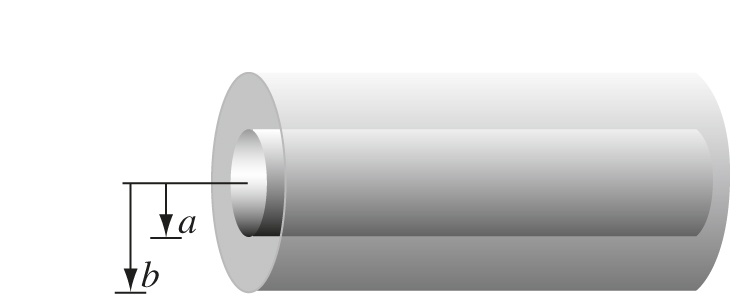
\includegraphics[width=0.25\textwidth]{figures/2_53.jpg} \hspace{0.1cm}
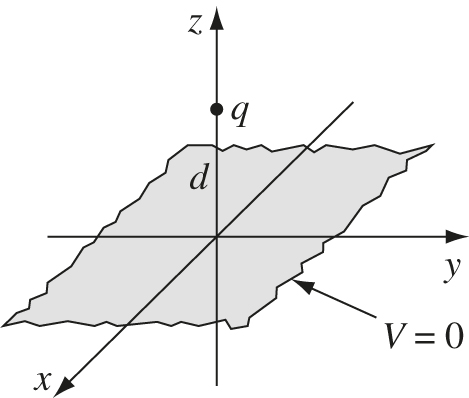
\includegraphics[width=0.19\textwidth]{figures/3_10.jpg}
\caption{\label{fig:1} (Left) A cylindrical coaxial cable with capacitance per unit length. (Right) A charge above a grounded conducting plane.}
\end{figure}

\section{Capacitance}

\begin{enumerate}
\item Consider the conductors in Fig. \ref{fig:1} (left).  Show that the capacitance per unit length is $C/l = 2\pi\epsilon_0/\ln(b/a)$. \\ \vspace{1.5cm}
\item Recall that the capacitance of two identical parallel conducting plates with area $A$ and separated by a distance $d$ is $C = \epsilon_0 A/d$.  Show that the stored energy at a potential difference $V$ is $W = (1/2) C V^2$. \\ \vspace{2.0cm}
\end{enumerate}

\section{Potentials}

\begin{enumerate}
\item \textbf{Uniqueness theorems}.  \textit{Uniqueness theorems} for \\ Laplace's equation ($\nabla^2 V=0$) and Poisson's equation ($\nabla^2 V = - \rho/\epsilon_0$) demonstrate that if a solution for the potential in a region is found, subject to boundary conditions and source charge distributions, it is the \textit{only} solution.  (a) How many solutions are there for the following differential equation?
\begin{equation}
\frac{d^2V}{dx^2} = 0
\end{equation}
(b) Suppose $V(0) = 1$ Volt, and $dV/dx = 2$ Volts per meter.  What is $V(3)$?  Is the formula you used to evaluate this the only solution? \\ \vspace{1cm}
\item Consider Fig. \ref{fig:1} (right).  A point charge $q$ is located a distance $z$ above the xy-plane, which is filled with a grounded conductor.  (a) Write equations that describe the boundary conditions. (b) Suppose, instead of a grounded conducting plane at $z=0$, there was a charge $-q$ a distance $-z$ below the xy-plane.  Does this configuration satisfy the boundary conditions of part (a)? (c) What is the potential $V(x,y,z)$ for the two charges?  Given the uniqueness theorem, this must be the \textit{only} solution.  Show that configuration of two point charges has the right units and limits.  \\ \vspace{3cm}
\item Recall that $\mathbf{E}_{\rm above} - \mathbf{E}_{\rm below} = \sigma/\epsilon_0 \hat{\mathbf{n}}$, which implies $\sigma = -\epsilon_0 (\partial V/\partial n)$ for Fig. \ref{fig:1} (right).  Calculate $\sigma(x,y)$ and the total charge.
\end{enumerate}

\end{document}
